\documentclass[a4paper,10pt]{article}

\usepackage[margin=1in]{geometry} 	% Setea el margen manualmente, todos iguales.
\usepackage[spanish]{babel} 		% {Con estos dos anda
\usepackage[utf8]{inputenc} 		% todo lo que es tildes y ñ}
\usepackage{fancyhdr} 			%{Estos dos son para
\usepackage{ulem}
\pagestyle{fancyplain} 			% el header copado}
\usepackage{color}			% Con esto puedo hacer la matufia de poner en color blanco un texto para engañar al formato
\usepackage{graphicx}	% Para insertar gráficos
\usepackage{array}			% Para usar arrays
\usepackage{hyperref}		% Para que tenga links el índice
\usepackage{lscape}         % Para apaisar figuras
\usepackage{ textcomp }

%\usepackage{datetime}	% Para agregar automáticamente fecha/hora de compilación y otras cosas

\lhead{Ingeniería de Software II} 	% {Con esto se usa el header copado. También está \chead para
\rhead{Big Cherry} 	% el centro y comandos para el pie de página, buscar fancyhdr}
\renewcommand{\footrulewidth}{0.4pt}
\lfoot{Facultad de Ciencias Exactas y Naturales}
\rfoot{Universidad de Buenos Aires}
%\rfoot{\textit{}}
\usepackage{amsfonts}	% para simbolos de reales, naturales, etc. se usa \mathbb{•} y la letra
\usepackage{amsmath}	% para \implies
%\usepackage{algorithm}
%\usepackage{algorithmic}
\usepackage{caratula}
\usepackage{pdfpages}

%%%%%%%%%%%%%%%%%%%%%%%%%%%%%%%%%%%%%
%      COMANDOS ÚTILES USADOS       %
%%%%%%%%%%%%%%%%%%%%%%%%%%%%%%%%%%%%%

% \section{title} 		Te hace un título ``importante'' en negrita, numerado. También está \subsection{title} y \subsubsection{title}.
% \begin{itemize}		Te hace viñetas.
%	\item esto es un item	Cambiar itemize por enumerate te hace una numeración.
% \end{itemize}

% \textbf{text} 		Te hace el texto en negrita (bold).
% \underline{text}		Te subraya el texto.

% \textsuperscript{text}	Te hace ``superindices'' con texto. En teoría subscript debería funcionar, pero se puede usar guion bajo entre llaves
% 				y signos peso para hacerlo como alternativa. Sino buscar.

% \begin{tabular}{cols} 	Es para hacer tablas. Se pone una c por cada columna deseada dentro de cols (si es que se desea centrada, l para justificar a 
%	a & b & c		izquierda, r a la derecha). Si se separa por espacios la tabla no tendrá líneas divisorias. Si se separa por | en lugar de 
% \end{tabular}			espacios, aparecerá una línea. Con || dos, y así. Luego para los elementos de las filas se escriben y se separan con ampersand (&).
%				Finalmente, para las líneas horizontales, se usa \hline para una linea en toda la tabla y \cline{i - j} te hace la linea desde
%				la celda i hasta la j, arrancando en 1.
%				Si en la columna se pone p(width) podés escribir un párrafo en la celda. Para hacer un enter con \\ no funciona porque te hace un
%				enter en la fila. Para eso se usa el comando \newline.
  
% \textcolor{color predefinido en palabras}{text}

%%%%%%%%%%%%%%%%%%%%%%%%%%%%%%%%%%%%%
%    FIN COMANDOS ÚTILES USADOS     %
%%%%%%%%%%%%%%%%%%%%%%%%%%%%%%%%%%%%%

\newcommand{\Gather}[1]{\begin{gather*}#1\end{gather*}}
%\newcommand{\Def}[1]{\textbf{Definición: }#1}
%\newcommand{\Prop}[1]{\textbf{Propiedad: }#1}
%\newcommand{\Teo}[1]{\textbf{Teorema: }#1}
\newcommand{\Obs}[1]{\textbf{Observación: }#1}
%\newcommand{\Amat}{A \in \mathbb{R}^{n\textnormal{x}n}}
\newcommand{\filtro}[1]{\textbf{\textit{#1}}}
\renewcommand{\labelenumii}{\theenumii}
\renewcommand{\theenumii}{\theenumi.\arabic{enumii}.}

\begin{document}

%%%%%%%%%%%%%%%%%%%%%%%%%%%
%			INICIO DE CARÁTULA			%
%%%%%%%%%%%%%%%%%%%%%%%%%%%

%% **************************************************************************
%
%  Package 'caratula', version 0.2 (para componer caratulas de TPs del DC).
%
%  En caso de dudas, problemas o sugerencias sobre este package escribir a
%  Nico Rosner (nrosner arroba dc.uba.ar).
%
% **************************************************************************



% ----- Informacion sobre el package para el sistema -----------------------

\NeedsTeXFormat{LaTeX2e}
\ProvidesPackage{caratula}[2003/4/13 v0.1 Para componer caratulas de TPs del DC]


% ----- Imprimir un mensajito al procesar un .tex que use este package -----

\typeout{Cargando package 'caratula' v0.2 (21/4/2003)}


% ----- Algunas variables --------------------------------------------------

\let\Materia\relax
\let\Submateria\relax
\let\Titulo\relax
\let\Subtitulo\relax
\let\Grupo\relax


% ----- Comandos para que el usuario defina las variables ------------------

\def\materia#1{\def\Materia{#1}}
\def\submateria#1{\def\Submateria{#1}}
\def\titulo#1{\def\Titulo{#1}}
\def\subtitulo#1{\def\Subtitulo{#1}}
\def\grupo#1{\def\Grupo{#1}}


% ----- Token list para los integrantes ------------------------------------

\newtoks\intlist\intlist={}


% ----- Comando para que el usuario agregue integrantes

\def\integrante#1#2#3{\intlist=\expandafter{\the\intlist
	\rule{0pt}{1.2em}#1&#2&\tt #3\\[0.2em]}}


% ----- Macro para generar la tabla de integrantes -------------------------

\def\tablaints{%
	\begin{tabular}{|l@{\hspace{4ex}}c@{\hspace{4ex}}l|}
		\hline
		\rule{0pt}{1.2em}Integrante & LU & Correo electr\'onico\\[0.2em]
		\hline
		\the\intlist
		\hline
	\end{tabular}}


% ----- Codigo para manejo de errores --------------------------------------

\def\se{\let\ifsetuperror\iftrue}
\def\ifsetuperror{%
	\let\ifsetuperror\iffalse
	\ifx\Materia\relax\se\errhelp={Te olvidaste de proveer una \materia{}.}\fi
	\ifx\Titulo\relax\se\errhelp={Te olvidaste de proveer un \titulo{}.}\fi
	\edef\mlist{\the\intlist}\ifx\mlist\empty\se%
	\errhelp={Tenes que proveer al menos un \integrante{nombre}{lu}{email}.}\fi
	\expandafter\ifsetuperror}


% ----- Reemplazamos el comando \maketitle de LaTeX con el nuestro ---------

\def\maketitle{%
	\ifsetuperror\errmessage{Faltan datos de la caratula! Ingresar 'h' para mas informacion.}\fi
	\thispagestyle{empty}
	\begin{center}
	\vspace*{\stretch{2}}
	{\LARGE\textbf{\Materia}}\\[1em]
	\ifx\Submateria\relax\else{\Large \Submateria}\\[0.5em]\fi
	\par\vspace{\stretch{1}}
	{\large Departamento de Computaci\'on}\\[0.5em]
	{\large Facultad de Ciencias Exactas y Naturales}\\[0.5em]
	{\large Universidad de Buenos Aires}
	\par\vspace{\stretch{3}}
	{\Large \textbf{\Titulo}}\\[0.8em]
	{\Large \Subtitulo}
	\par\vspace{\stretch{3}}
	\ifx\Grupo\relax\else\textbf{\Grupo}\par\bigskip\fi
	\tablaints
	\end{center}
	\vspace*{\stretch{3}}
	\newpage}





\materia{Ingeniería de Software 2}
\submateria{Segundo Cuatrimestre de 2014}
\titulo{Trabajo Práctico 2 \\ Big Data \& Agro - Big Cherrys}

\grupo{Grupo 1}
\integrante{Giordano, Mauro}{125/10}{mauro.foxh@gmail.com}
\integrante{Iglesias, Axel}{79/10}{axeligl@gmail.com}
\integrante{Lascano, Nahuel}{476/11}{laski.nahuel@gmail.com}
\integrante{Lazzaro, Leonardo}{147/05}{lazzaroleonardo@gmail.com}

\begin{titlepage}
\maketitle
\thispagestyle{empty}
\end{titlepage} 

%%%%%%%%%%%%%%%%%%%%%%%%%%%
%				FIN DE CARÁTULA			%
%%%%%%%%%%%%%%%%%%%%%%%%%%%

\tableofcontents
%\clearpage

%%%%%%%%%%%%%%%%%%%%%%%%%%%
%					DESARROLLO				%
%%%%%%%%%%%%%%%%%%%%%%%%%%%

\section{Introducción}

En el presente trabajo se aborda la extensión del diseño presentado en el TP1, debiendo ahora plantear un sistema de cultivo de muchas plantas en grandes extensiones de terreno y para muchos clientes. Dada esta nueva situación, aparecen varios stakeholders que, por su colaboración en el proyecto proveyendo logística o servicios, o por su intención de consumo, imponen distintos requerimientos que sumados a los técnicos desembocan en la contemplación de diversos riesgos y atributos de calidad.\\
Aquí se presenta una planificación de las fases de \textit{elaboración} y \textit{construcción} de la metodología UP, asumiendo que la fase \textit{inception} ya se ha desarrollado. En esta primera etapa se han presentado las ideas para la formulación del proyecto BigCherry, se han establecido los requerimientos y recursos disponibles, y se ha llevado a cabo el QAW del cual se desprendieron algunos atributos de calidad esperados en el producto final.

\section{Casos de Uso}

\subsection{Asignación de CU}

Para comenzar a trabajar sobre la planificación del proyecto se identificó un conjunto de casos de uso que cubriera la mayoría de las funcionalidades que se desprenden de los requerimientos obtenidos. Los mismos se organizaron en seis iteraciones, distribuidas a lo largo de las fases de elaboración y construcción de la metodología UP. La división de los CU en las distintas iteraciones y la organización de las mismas estuvo pautada por las necesidades manifestadas por los stakeholders y un incremento de funcionalidad, partiendo del núcleo más importante y revistiendo la aplicación a lo largo del tiempo de lógica menos prioritaria.\\
\indent Dado que la primera iteración ya contaba con un tiempo fijado (3 semanas), se determinó trabajar en este tiempo en la comunicación con la red pública de drones (ya que el Ministerio exigía que esto estuviera implementado en los primeros dos meses), la recepción y procesamiento de las imágenes, la traducción de estos datos en mediciones de los indicadores de estado de los cultivos y una mínima interacción con actuadores. Para las siguientes iteraciones se adjudicaron casos de uso que totalizaran una cantidad de tiempo similar y que implicaran una evolución coherente y funcional de la aplicación. Por ejemplo, para la segunda iteración se asignaron los casos de uso relacionados con la programación de seguimiento de cultivos, el monitoreo de la salud de las plantas y la comunicación con las estaciones climatológicas, mientras que la encrptación de datos se diagramó en la órbita de la sexta y última iteración.\\
\indent Parte de este cronograma fue también regido por el análisis de riesgos, presentado en la \textbf{SECCION}, el cual se vio alimentado por los requerimientos iniciales y por las intervenciones de los distintos stakeholders en el QAW. De esta manera, dado que el riesgo más importante resultó ser la correcta implementación de la comunicación con la red pública de drones, se decidió incluir este desarrollo dentro de la primera iteración, de casi un mes de duración, para garantizar que haya el suficiente tiempo para llevar adelante esta tarea dentro del marco de tiempo requerido.

\clearpage

\subsection{Iteraciones}

\textbf{Primera iteración} [3 semanas]
	\begin{enumerate}
		\item Accediendo a la red pública de drones
		\item Recibiendo imágenes de los drones
		\item Procesando datos de bandas espectrales de las fotografías
		\item Interactuando con actuadores
	\end{enumerate}

\textbf{Segunda iteración} [2 semanas]
	\begin{enumerate}
		\item Generando mediciones de estado del terreno / cultivos a partir de fotos procesadas
		\item Monitoreando el estado de salud de las plantas
		\item Obteniendo información del clima a partir de las micro-estaciones climatológicas del INTA.
		\item Calculando decisión según información recolectada y plan maestro
	\end{enumerate}

\textbf{Tercera iteración} [2 semanas]
	\begin{enumerate}
		\item Iniciando seguimiento de cultivos / región
		\item Incorporando nuevas especies de cultivo (ABM Cultivo)
		\item Consultando planes maestros de cultivo provistos por el INTA / organismos privados (ABM Plan)
		\item Consultando estado de los cultivos
		\item Accediendo a la red privada de drones
	\end{enumerate}

\textbf{Cuarta iteración} [2 semanas]
	\begin{enumerate}
		\item Supervisando acciones ordenadas a actuadores
		\item Agregando muestreo manual del estado de los cultivos / terreno
		\item Visualizando el mapa del estado del terreno
		\item Personalizando plan maestro de cultivo
		\item Agregando nuevos actuadores (ABM Actuador)
	\end{enumerate}

\textbf{Quinta iteración} [2 semanas]
	\begin{enumerate}
		\item Logueando eventos del sistema
		\item Autenticando usuario (ABM Usuario)
		\item Autorizando usuario (ABMs Rol y Permiso)
		\item Revisando registro de eventos
	\end{enumerate}

\textbf{Sexta iteración} [2 semanas]
	\begin{enumerate}
		\item Manejando fallas de servidores de INTA
		\item Descargando fotos offline de dron
		\item Organizando información almacenada entre nodos ArSat
		\item Encriptando / desencriptando información a almacenar
	\end{enumerate}

\clearpage

\subsection{Síntesis CU Primera iteración}
		
\begin{enumerate}
	\item \textbf{Accediendo a la red pública de drones}
	Se refiere a la conexión y comunicación con la red estatal de drones. BigCherry debe poder iniciar una sesión dentro de la red y realizar peticiones de imágenes para ciertas coordenadas. Debe poder enviar los mensajes acorde a la especificación de la API de la red y a su vez debe poder interpretar los distintos mensajes que ésta le envía, sean de comportamiento normal o error. Esto debe permitir, además, la parametrización de los pedidos y el acceso a otros datos de los drones como disponibilidad, tiempo estimado de envío de la información, etc.

	\item \textbf{Recibiendo imágenes de los drones}
	Una vez satisfecho el pedido de imágenes aéreas, el sistema debe poder recibir las mismas sin errores y almacenarlas correctamente para su posterior procesamiento. Es importante que pueda manejar la recepción de muchas imágenes en simultáneo y que esto no afecte transimisión de otros datos con el resto de los drones.

	\item \textbf{Procesando datos de bandas espectrales de las fotografías}
	Al analizar las imágenes se deben aplicar distintos filtros para obtener datos del suelo como temperatura, humedad, salinidad del agua y otros indicadores pertinentes a la salud de las plantas. Ademśas se deben determinar posibles problemas como fotografías corruptas, mal tomadas (con obstáculos) o que presenten otro tipo de anomalías. La salida de este procesamiento debe almacenarse acorde al input procesado para posteriores consultas.

	\item \textbf{Interactuando con actuadores} 
	Este CU refiere a la interacción de BigCherry con los actuadores registrados, ya sean pulverizadoras, cosechadoras, sistemas de riego o fertilización, etc. Deben poder enviarse mensajes con directivas para que éstos lleven a cabo a través del protocolo de comunicación que maneje cada dispositivo.
\end{enumerate}

\subsection{Detalle Primera iteración}

\begin{itemize}
\item Identificación: E1
\item Tipo de iteración: Elaboración
\item Tareas:
	\begin{enumerate}
	\item Refinamiento de objetivos y requerimientos
	\item QAW con stakeholders y equipo
	\item Análisis de riesgos
	\item Reconocimiento de casos de uso
	\item División de CU en iteraciones según prioridad
	\item Estimación de tiempos de CU
	\item Análisis de escenarios y atributos de calidad del sistema
	\item Diseño de arquitectura
	\item Realización de tareas de CU1
	\item Realización de tareas de CU2
	\item Realización de tareas de CU3
	\item Realización de tareas de CU4	
	\end{enumerate}
\end{itemize}


\begin{landscape}
\begin{table}[ht]
\caption{Iteraciones}
\centering 
\begin{tabular}{c c c c}
\hline
Nombre                                                      & Inicio estimado & Fin estimado & Duración \\
\hline
Inicio                                                      & Vie 24/10/14    & Vie 24/10/14 & 0 días   \\
ABM Región                                                  & Vie 24/10/14    & Vie 24/10/14 & 1 día    \\
ABM Drones                                                  & Vie 24/10/14    & Vie 24/10/14 & 1 día    \\
ABM Usuarios                                                & Vie 24/10/14    & Lun 27/10/14 & 2 días   \\
ABM Perfiles de usuario                                     & Mar 28/10/14    & Vie 31/10/14 & 4 días   \\
Recibir imágenes drones                                     & Lun 27/10/14    & Mié 29/10/14 & 3 días   \\
Procesamiento imágenes y armado mapas                       & Jue 30/10/14    & Mar 11/11/14 & 9 días   \\
Login Usuario                                               & Mar 28/10/14    & Mié 29/10/14 & 2 días   \\
Deslogueo del sistema                                       & Mié 12/11/14    & Mié 12/11/14 & 1 día    \\
Vista Mapa de Región                                        & Mié 12/11/14    & Jue 20/11/14 & 7 días   \\
Tests Login con perfiles                                    & Jue 13/11/14    & Mié 19/11/14 & 5 días   \\
Test funcionales para mapas con screenshots                 & Vie 21/11/14    & Jue 27/11/14 & 5 días   \\
Pruebas del procesamiento de imágenes                       & Mié 12/11/14    & Jue 13/11/14 & 2 días   \\
Pruebas con drones verdaderos                               & Vie 28/11/14    & Jue 04/12/14 & 5 días   \\
Fix bug                                                     & Lun 08/12/14    & Mar 09/12/14 & 2 días   \\
Preparación demo para ministerio agricultura                & Mié 10/12/14    & Mié 10/12/14 & 1 día    \\
Demo                                                        & Mié 10/12/14    & Mié 10/12/14 & 0 días   \\
ABM Sensores                                                & Jue 11/12/14    & Jue 11/12/14 & 1 día    \\
Obtención datos INTA                                        & Vie 12/12/14    & Jue 18/12/14 & 5 días   \\
Cálculo del estado del cultivo                              & Mié 24/12/14    & Vie 26/12/14 & 3 días   \\
Vista para mostrar salud plantas                            & Lun 29/12/14    & Mié 31/12/14 & 3 días   \\
Testing nuevas features                                     & Jue 01/01/15    & Jue 01/01/15 & 1 día    \\
Fix bugs                                                    & Vie 02/01/15    & Lun 05/01/15 & 2 días   \\
ABM Superusuario Planes                                     & Mar 06/01/15    & Mar 06/01/15 & 1 día    \\
ABM Cultivo                                                 & Mié 07/01/15    & Mié 07/01/15 & 1 día    \\
Permitir personalización de planes                          & Jue 08/01/15    & Lun 12/01/15 & 3 días   \\
Testing Planes                                              & Mar 13/01/15    & Mié 14/01/15 & 2 días   \\
ABM Clientes                                                & Mar 06/01/15    & Mar 06/01/15 & 1 día    \\
Desarrollo Perfil Cliente                                   & Jue 08/01/15    & Vie 09/01/15 & 2 días   \\
Testing usuarios clientes                                   & Lun 12/01/15    & Mar 13/01/15 & 2 días   \\
Fix bugs                                                    & Mié 14/01/15    & Vie 16/01/15 & 3 días   \\
ABM Actuador                                                & Vie 16/01/15    & Lun 19/01/15 & 2 días   \\
Envio de comandos a actuadores                              & Mar 20/01/15    & Lun 26/01/15 & 5 días   \\
Grilla de órdenes por enviar                                & Mar 20/01/15    & Jue 22/01/15 & 3 días   \\
Cancelación de órdenes para actuadores                      & Vie 23/01/15    & Mar 27/01/15 & 3 días   \\
\end{tabular}
\end{table}
\end{landscape}

\begin{landscape}
\begin{table}[ht]
\caption{Iteraciones}
\centering 
\begin{tabular}{c c c c}
\hline
Nombre                                                      & Inicio estimado & Fin estimado & Duración \\
\hline
Testing                                                     & Mié 28/01/15    & Vie 30/01/15 & 3 días   \\
Fix bugs                                                    & Lun 02/02/15    & Lun 02/02/15 & 1 día    \\
Grilla con los registros de decisiones tomadas              & Mar 03/02/15    & Jue 05/02/15 & 3 días   \\
Grilla con los usos en hectáreas usadas de la red privada   & Mar 03/02/15    & Mié 04/02/15 & 2 días   \\
Detección de fallas con el INTA                             & Mar 03/02/15    & Mié 04/02/15 & 2 días   \\
Reporte de fallas con el INTA                               & Jue 05/02/15    & Vie 06/02/15 & 2 días   \\
Testing                                                     & Lun 09/02/15    & Mié 11/02/15 & 3 días   \\
Fix bugs                                                    & Mié 11/02/15    & Vie 13/02/15 & 3 días   \\
Testing funcionales                                         & Lun 23/02/15    & Jue 26/02/15 & 4 días   \\
Fix bugs                                                    & Vie 27/02/15    & Lun 02/03/15 & 2 días   \\
Deploy en produccion                                        & Mar 03/03/15    & Mié 04/03/15 & 2 días   \\
Prueba de humo                                              & Jue 05/03/15    & Jue 05/03/15 & 1 día    \\
Fin                                                         & Vie 24/10/14    & Vie 24/10/14 & 0 días   \\

\end{tabular}
\end{table}
\end{landscape}
\section{Análisis de Riesgos}

\textbf{Interfaz con los drones en dos meses}
\begin{itemize}
 \item \textsl{Descripci\'on}: 
 \item \textsl{Probabilidad}: 
 \item \textsl{Impacto}: 
 \item \textsl{Exposición}: 
 \item \textsl{Mitigación}: 
 \item \textsl{Plan de Contingencia} : 
\end{itemize}
\textbf{Disponibilidad usando la red estatal}
\begin{itemize}
 \item \textsl{Descripci\'on}: 
 \item \textsl{Probabilidad}: 
 \item \textsl{Impacto}: 
 \item \textsl{Exposición}: 
 \item \textsl{Mitigación}: 
 \item \textsl{Plan de Contingencia} : 
\end{itemize}
\textbf{Servidores del INTA inestables}
\begin{itemize}
 \item \textsl{Descripci\'on}: 
 \item \textsl{Probabilidad}: 
 \item \textsl{Impacto}: 
 \item \textsl{Exposición}: 
 \item \textsl{Mitigación}: 
 \item \textsl{Plan de Contingencia} : 
\end{itemize}
\textbf{Demasiado volumen de informaci\'on }
\begin{itemize}
 \item \textsl{Descripci\'on}: 
 \item \textsl{Probabilidad}: 
 \item \textsl{Impacto}: 
 \item \textsl{Exposición}: 
 \item \textsl{Mitigación}: 
 \item \textsl{Plan de Contingencia} : 
\end{itemize}
\textbf{Uso de servidores p\'ublicos}
\begin{itemize}
 \item \textsl{Descripci\'on}: 
 \item \textsl{Probabilidad}: 
 \item \textsl{Impacto}: 
 \item \textsl{Exposición}: 
 \item \textsl{Mitigación}: 
 \item \textsl{Plan de Contingencia} : 
\end{itemize}
\textbf{Auditabilidad en todas las decisiones tomadas para validar imparcialidad}
\begin{itemize}
 \item \textsl{Descripci\'on}: 
 \item \textsl{Probabilidad}: 
 \item \textsl{Impacto}: 
 \item \textsl{Exposición}: 
 \item \textsl{Mitigación}: 
 \item \textsl{Plan de Contingencia} : 
\end{itemize}
\textbf{zonas relefadas por motivos politicos alegando motivos t\'ecnicos}
\begin{itemize}
 \item \textsl{Descripci\'on}: 
 \item \textsl{Probabilidad}: 
 \item \textsl{Impacto}: 
 \item \textsl{Exposición}: 
 \item \textsl{Mitigación}: 
 \item \textsl{Plan de Contingencia} : 
\end{itemize}

\textbf{Errores en las comunicaciones}
\begin{itemize}
 \item \textsl{Descripci\'on}: Pueden surgir errores en la comunicación con los servidores del \textbf{INTA}
 \item \textsl{Probabilidad}: Media
 \item \textsl{Impacto}: Media
 \item \textsl{Exposición}: Media
 \item \textsl{Mitigación}: Detectar fallas en la comunicación para poder reportar y seguir con el normal funcionamineto.
 \item \textsl{Plan de Contingencia} : Utilizar informaci\'on de sensores e imágenes de drones para poder calcular resultados similares a los del \textbf{INTA}.
\end{itemize}

\textbf{Cobertura de conexión}
\begin{itemize}
 \item \textsl{Descripci\'on}: Problemas de conectividad en zonas sin acceso a internet u otras redes de comunicación.
 \item \textsl{Probabilidad}: Alta
 \item \textsl{Impacto}: Media
 \item \textsl{Exposición}: Media
 \item \textsl{Mitigación}: El sistema llevaría un historial con fecha de datos externos y detectaría cuándo los datos son viejos usando un reloj interno.
 \item \textsl{Plan de Contingencia}: Permitir la carga manual de datos por medio de importación de archivos u otras fuentes.
\end{itemize}

\textbf{Vulnerabilidades en la seguridad}
\begin{itemize}
 \item \textsl{Descripci\'on}: Cliente puede ver datos de otro cliente.
 \item \textsl{Probabilidad}: Baja
 \item \textsl{Impacto}: Alto
 \item \textsl{Exposición}: Media
 \item \textsl{Mitigación}: Realizar test para probar casos de borde con los cuentas de clientes. Pagar a una consultora de seguridad para pruebas tercerizadas.
 \item \textsl{Plan de Contingencia}: Permitir el apagado rápido del sistema en caso de detecci\'on de problemas de seguridad. Guardar en logs las operaciones realizadas para cada dominio / cliente / empresa.
\end{itemize}

\textbf{Aumento de costos por utilizar la red privada de drones}
\begin{itemize}
 \item \textsl{Descripci\'on}: Se utiliza mucho la red privada de drones en vez de la pública.
 \item \textsl{Probabilidad}: Media
 \item \textsl{Impacto}: Alto
 \item \textsl{Exposición}: Alto
 \item \textsl{Mitigación}: El sistema calcularía cada cierto intervalo el consumo por hect\'areas.
 \item \textsl{Plan de Contingencia} : Desactivar la red privada en caso de susperar algún límite de uso diario, mensual, etc. Enviar alertar al administrador del sistema. Si no logra acceder a la red pública pasa al caso de falta de conectividad y se aplica el plan 
\end{itemize}

\clearpage

\textbf{Delays en accionar de actuadores}
\begin{itemize}
 \item \textsl{Descripci\'on}: Demora al enviar acciones a los actuadores.
 \item \textsl{Probabilidad}: Media
 \item \textsl{Impacto}: Alta
 \item \textsl{Exposición}: Alta
 \item \textsl{Mitigación}: En el sistema se usarán actuadores que confirman la recepci\'on de acciones.
 \item \textsl{Plan de Contingencia}: Se chequeará que las acciones fueron recibidas por los actuadores y en caso de timeout se reenviarán. Ante la primera falla se le avisar\'a al administrador / encargado.
\end{itemize}

\textbf{Problemas con almacenamiento}
\begin{itemize}
 \item \textsl{Descripci\'on}: Volumen de informaci\'on muy grande.
 \item \textsl{Probabilidad}: Media
 \item \textsl{Impacto}: Alto
 \item \textsl{Exposición}: Alto
 \item \textsl{Mitigación}: Utilizar algoritmos para comprimir los datos.
 \item \textsl{Plan de Contingencia}: Monitorear el trafico de la red y espacio de disco en los nodos de \textbf{ArSAT}. Rediseñar parte de la persistencia para evitar redundancia de datos innecesaria.
\end{itemize}

\section{Escenarios}
\subsection{Disponibilidad}
\textbf{Motivación}
\begin{itemize}
 \item Del Ministerio de Agricultura se quiere que el sistema funcione ``todo el tiempo, en todos los climas''.
 \item A su vez, se niega a utilizar la red privada salvo que sea estrictamente necesario.
 \item El Repesentante de Entidades y Productores Agrícolas quiere poder usarlo ``en todo el país en todo momento''.
 \item Defensa al Consumidor coincide, el sistema debe funcionar ``en todo el país sin problemas''.
 \item Los drones de la red privadad mejoran la disponibilidad.
 \item El sistema se usa en una zona donde no se puede garantizar conectivdad permanente entre los distntos artefactos.
\end{itemize}


\begin{tabular}{| l || p{12cm} |}
\hline 
\textbf{Descripci\'on} & La red de drones pública podría tener problemas. En ese caso, hay que pasar a usar la red privada. \\
\hline 
\textbf{Fuente} & Sistema central \\
\hline 
\textbf{Estimulo} & Un pedido de foto de una posición \\
\hline 
\textbf{Artefacto} & Sistema de comunicación con drones \\
\hline 
\textbf{Entorno} & Conexión con la red de drones pública caída \\
\hline 
\textbf{Respuesta} & La foto se saca de todos modos usando la red privada \\
\hline 
\textbf{Medici\'on} & 9 de cada 10 veces la foto se saca correctamente \\
\hline 
\end{tabular}

\medskip

\begin{tabular}{| l || p{12cm} |}
\hline 
\textbf{Descripci\'on} & Si la red pública de drones se reestablece, debo priorizarla para ahorrar recursos estatales. \\
\hline 
\textbf{Fuente} & Sistema central \\
\hline 
\textbf{Estimulo} & Un pedido de foto de una posición \\
\hline 
\textbf{Artefacto} & Sistema de comunicación con drones \\
\hline 
\textbf{Entorno} & Conexión con la red de drones pública funcionando correctamente \\
\hline 
\textbf{Respuesta} & La foto se saca usando la red pública \\
\hline 
\textbf{Medici\'on} & La foto se obtiene correctamente \\
\hline 
\end{tabular}

\medskip

\begin{tabular}{| l || p{12cm} |}
\hline 
\textbf{Descripci\'on} & Los servidores del $INTA$ para el pronóstico del tiempo son nuevos y podr\'ian fallar. Se deben comunicar las fallas de los servidores al $INTA$. \\
\hline 
\textbf{Fuente} & Comunicador con los servidores del $INTA$\\
\hline 
\textbf{Estimulo} & Los servidores del $INTA$ fallan\\
\hline 
\textbf{Artefacto} & Sistema de comunicación \\
\hline 
\textbf{Entorno} & Normal \\
\hline 
\textbf{Respuesta} & Se envía un mail al responsable técnico del $INTA$ anunciando la falla \\
\hline 
\textbf{Medici\'on} & El mail se envía en los siguientes 5 minutos \\
\hline 
\end{tabular}

\medskip

\begin{tabular}{| l || p{12cm} |}
\hline 
\textbf{Descripci\'on} & Tanto el Responsable T\'ecnico de ArSAT como el Representante de Entidades y Productores Agr\'icolas están preocupados por que el volumen de informaci\'on sea demasiado. El sistema debe responder bien ante grandes cantidades de datos. \\
\hline 
\textbf{Fuente} & Interfaz con los drones \\
\hline 
\textbf{Estimulo} & Se reciben las imágenes de los drones \\
\hline 
\textbf{Artefacto} & Sistema de procesamiento de imágenes \\
\hline 
\textbf{Entorno} & Normal \\
\hline 
\textbf{Respuesta} & Se procesan las imágenes correctamente \\
\hline 
\textbf{Medici\'on} & En un 99,999\% de los casos se procesan correctamente las imágenes \\
\hline 
\end{tabular}

\subsection{Performance}
\textbf{Motivación}
\begin{itemize}
 \item El Ministerio de Agricultura quiere que el sistema funcione rápido porque sino podría arruinar cosechas.
 \item El Responsable Técnico prefiere usar los drones privados porque garantizan mayor rapidez.
 \item Pero el Ministerio de Agricultura se opone.
 \item El enunciado especifica que la interacción con los actuadores debe ser rápida.
\end{itemize}

\begin{tabular}{| l || p{12cm} |}
\hline 
\textbf{Descripci\'on} & La interacción con los actuadores debe ser rápida \\
\hline 
\textbf{Fuente} & Interfaz con los actuadores \\
\hline 
\textbf{Estimulo} & Se envía una órden de riego \\
\hline 
\textbf{Artefacto} & Manejador de los actuadores \\
\hline 
\textbf{Entorno} & Normal \\
\hline 
\textbf{Respuesta} & Los actuadores riegan la cosecha \\
\hline 
\textbf{Medici\'on} & El riego comienza a los 20 segundos de enviada la órden \\
\hline 
\end{tabular}

\medskip

\begin{tabular}{| l || p{12cm} |}
\hline 
\textbf{Descripci\'on} & Se debe priorizar el uso de drones públicos, pero pasar a los drones privados en caso de que los públicos tarden en responder \\
\hline 
\textbf{Fuente} & Interfaz con los drones \\
\hline 
\textbf{Estimulo} & Una respuesta de la red de drones pública toma más de 5 segundos \\
\hline 
\textbf{Artefacto} & Sistema de comunicación con drones \\
\hline 
\textbf{Entorno} & Normal \\
\hline 
\textbf{Respuesta} & Se empieza a utilizar la red de drones privada \\
\hline 
\textbf{Medici\'on} & El cambio del sistema se realiza en el 99\% de los casos \\
\hline 
\end{tabular}


\subsection{Seguridad}
\textbf{Motivación}
\begin{itemize}
 \item El Responsable T\'ecnico de ArSAT quiere ``un esquema serio de accesos y permisos'' para los usuarios.
 \item El Representante de Entidades y Productores Agr\'icolas considera fundamental que los planes maestros y datos de seguimiento sean seguros y confidenciales.
 \item Defensa al Consumidor quiere asegurar confidencialidad de todos los datos involucrados.
\end{itemize}

\begin{tabular}{| l || p{12cm} |}
\hline 
\textbf{Descripci\'on} & Un atacante debe ser rechazado \\
\hline 
\textbf{Fuente} & Sistema de planes maestros \\
\hline 
\textbf{Estimulo} & Un usuario intenta consultar un plan maestro que no le pertenece \\
\hline 
\textbf{Artefacto} & Gestor de credenciales \\
\hline 
\textbf{Entorno} & Normal \\
\hline 
\textbf{Respuesta} & Se rechaza la solicitud y se guarda un registro del intento \\
\hline 
\textbf{Medici\'on} & La solicitud se rechaza un 99,99\% de las veces \\
\hline 
\end{tabular}

\medskip

\begin{tabular}{| l || p{12cm} |}
\hline 
\textbf{Descripci\'on} & Un usuario correctamente identificado debe poder acceder a sus datos \\
\hline 
\textbf{Fuente} & Sistema de planes maestros \\
\hline 
\textbf{Estimulo} & Un usuario intenta consultar sus propios planes maestros \\
\hline 
\textbf{Artefacto} & Gestor de credenciales \\
\hline 
\textbf{Entorno} & Normal \\
\hline 
\textbf{Respuesta} & Se permite al usuario acceder \\
\hline 
\textbf{Medici\'on} & La solicitud se acepta un 99,99\% de las veces \\
\hline 
\end{tabular}

\subsubsection{Auditabilidad}
\textbf{Motivación}
\begin{itemize}
 \item El Representante de Entidades y Productores Agr\'icolas quiere poder supervisar las órdenes enviadas a los actuadores.
 \item Defensa al Consumidor quiere validar la imparcialidad del sistema, para lo cual quiere poder auditar todas las decisiones tomadas.
 \item También quiere asegurarse que los drones no serán utilizados para espiar a la población, con lo cual quiere poder conocer las instrucciones que se le dan y la información que devuelven.
 \item Sin embargo esto entra en conflicto con atributos de disponibilidad y performance juzgados más prioritarios (por ejemplo, la saturación de los servidores del $INTA$).
 \item Concluimos que se guardará siempre registro de las decisiones humanas (por ser las más importantes) y de las órdenes enviadas a los actuadores cuando el sistema tenga espacio suficiente.
\end{itemize}

\begin{tabular}{| l || p{12cm} |}
\hline 
\textbf{Descripci\'on} & Se podrán auditar las decisiones tomadas por personas \\
\hline 
\textbf{Fuente} & Interfaz de configuración \\
\hline 
\textbf{Estimulo} & Un usuario cambia un plan maestro \\
\hline 
\textbf{Artefacto} & Sistema de logging \\
\hline 
\textbf{Entorno} & Normal \\
\hline 
\textbf{Respuesta} & Se guarda un log del acceso y del cambio realizado \\
\hline 
\textbf{Medici\'on} & El log se guarda correctamente en un 99,99\% de los casos \\
\hline 
\end{tabular}

\medskip

\begin{tabular}{| l || p{12cm} |}
\hline 
\textbf{Descripci\'on} & Se podrán auditar las órdenes enviadas a los actuadores \\
\hline 
\textbf{Fuente} & Comunicación con la red de drones \\
\hline 
\textbf{Estimulo} & Se envía un pedido de captura de imágenes a una red \\
\hline 
\textbf{Artefacto} & Sistema de logging \\
\hline 
\textbf{Entorno} & Disco rígido al 90\% de su capacidad \\
\hline 
\textbf{Respuesta} & Se descarta el log de la orden enviada \\
\hline 
\textbf{Medici\'on} & El disco guarda únicamente los resultados de la orden \\
\hline 
\end{tabular}


\subsection{Modificabilidad}
\textbf{Motivación}
\begin{itemize}
 \item El Representante de Entidades y Productores Agr\'icolas quiere poder agregar nuevos actuadores sin mucha dificultad
\end{itemize}

\begin{tabular}{| l || p{12cm} |}
\hline 
\textbf{Descripci\'on} & Se pueden agregar actuadores fácilmente \\
\hline 
\textbf{Fuente} & Interfaz de configuración \\
\hline 
\textbf{Estimulo} & Un usuario desea agregar un nuevo actuador \\
\hline 
\textbf{Artefacto} & Panel de configuración de actuadores \\
\hline 
\textbf{Entorno} & Normal \\
\hline 
\textbf{Respuesta} & Se agrega el nuevo actuador correctamente \\
\hline 
\textbf{Medici\'on} & No hace falta modificar código del sistema \\
\hline 
\end{tabular}

\subsection{Usabilidad}
\textbf{Motivación}
\begin{itemize}
 \item El Representante de Entidades y Productores Agr\'icolas quiere que el sistema sea f\'acil de usar para todos los productores y los distintos tipos de perfiles
\end{itemize}

\begin{tabular}{| l || p{12cm} |}
\hline 
\textbf{Descripci\'on} & Un usuario debe poder consultar el estado de sus plantas fácilmente \\
\hline 
\textbf{Fuente} & Interfaz web del sistema \\
\hline 
\textbf{Estimulo} & Un usuario quiere consultar el estado de las plantas \\
\hline 
\textbf{Artefacto} & Interfaz web \\
\hline 
\textbf{Entorno} & Normal \\
\hline 
\textbf{Respuesta} & Se presentan al usuario las plantas presentes en sus campos junto con su información \\
\hline 
\textbf{Medici\'on} & No se necesitan más de tres clics para acceder a la información \\
\hline 
\end{tabular}
\include{justificacion_arq}
\section{Arquitectura}

En esta sección presentamos y analizamos la arquitectura diseñada para resolver las funcionalidades requeridas, conciliando a la vez las necesidades presentadas por los atributos de calidad y el análisis de riesgos.

\subsection{Comunicación con Drones}

Para el monitoreo de los cultivos se utilizan drones que toman fotografías de los terrenos, las cuales se procesan para extraer las mediciones necesarias sobre el estado de salud de las plantas.  Para esto, se cuenta con un componente dedicado a la comunicación con las interfaces de manejo de drones que nos proveen tanto el Ministerio como la empresa privada. Por defecto se prioriza la utilización del sistema de drones estatales, mientras que en caso de no responder a los pedidos se utiliza la red privada. Para atacar el problema de que los drones no tengan conectividad - y no se puedan recibir las imágenes tomadas por los mismos - se proveen repositorios temporales de imágenes en los nodos distribuidos de ArSat para que los aparatos descarguen las fotos tomadas. Luego, esta información se replica y reorganiza de acuerdo a la ubicación del acceso más frecuente.\\
\indent El componente encargado del pedido de imágenes busca en el repositorio de pedidos y, gracias al repositorio de geolocalización, envía la latitud y longitud que se desea analizar. A medida que se reciben las imágenes, se pasan al geolocalizador utilizando una cola que se encarga de identificar el tipo de cultivo analizando las imágenes y usando la información del repositorio de geolocalizaciones. Este componente se encarga también de descartar las imágenes erróneas que no permitan un posterior análisis correcto. El repositorio contiene información ingresada por los usuarios sobre la localización de las plantaciones, así como su estado. Esta información se utiliza para comparar con el análisis que haga el geolocalizador y poder verificar de qué plantación se trata. Una vez taggeada, la imagen se envía a los analizadores que trabajan en paralelo para reconocer la temperatura, el estado del suelo y la salinidad del agua. Eventualmente podrían agregarse más filtros para que analicen otras bandas espectrales de las fotos. Vale observar que este conjunto de componentes (los analizadores y el geolocalizador) tienen varias instancias corriendo en simultáneo para mejorar la performance. Luego de esto se procede a unificar los resultados, comprimir las imágenes tomadas y guardar en el repo de información de manera encriptada.\\

\begin{figure}[h!]
  \centering
  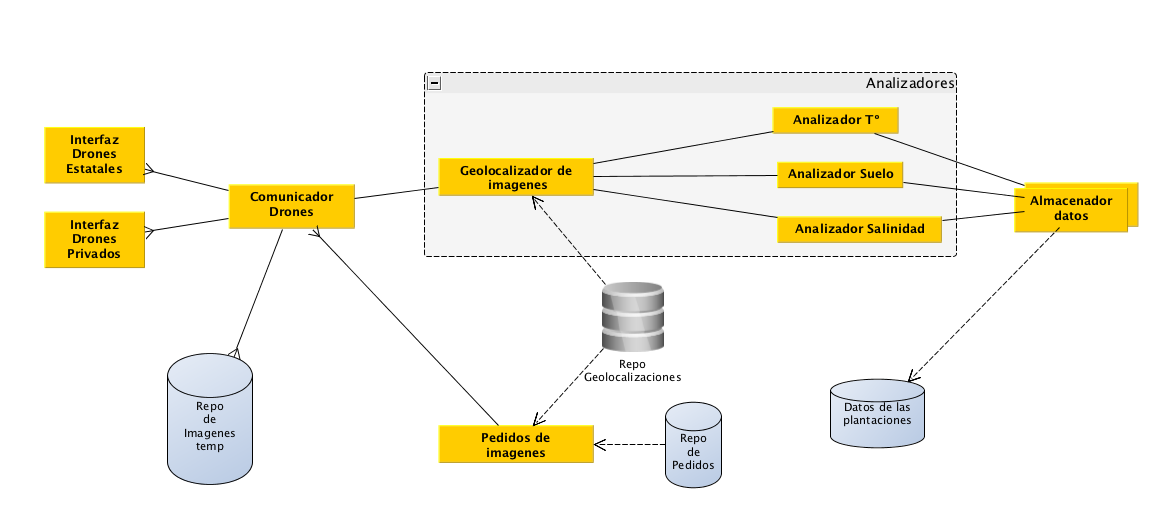
\includegraphics[width=1\textwidth]{./images/arq_drones.png}
  \caption{Arquitectura de comunicación con drones y procesamiento de imágenes}
  \label{fig:clases4}
\end{figure}

\subsection{Comunicación con estaciones meteorológicas}

El mecanismo es bastante similar a la comunicación con drones. Existe un repositorio de pedidos de clima que puede haber sido poblado por el usuario o por el sistema de monitoreo automático. El comunicador de estación meteorológica establece el pedido a la interfaz meteorológica definida y luego envía el paquete usando una cola al analizador, quien luego se lo envía al almacenados de datos que lo agrega al repo.

En caso de que la estación meteorológica no conteste, se envía un mail informando de este problema.

\begin{figure}[h!]
  \centering
  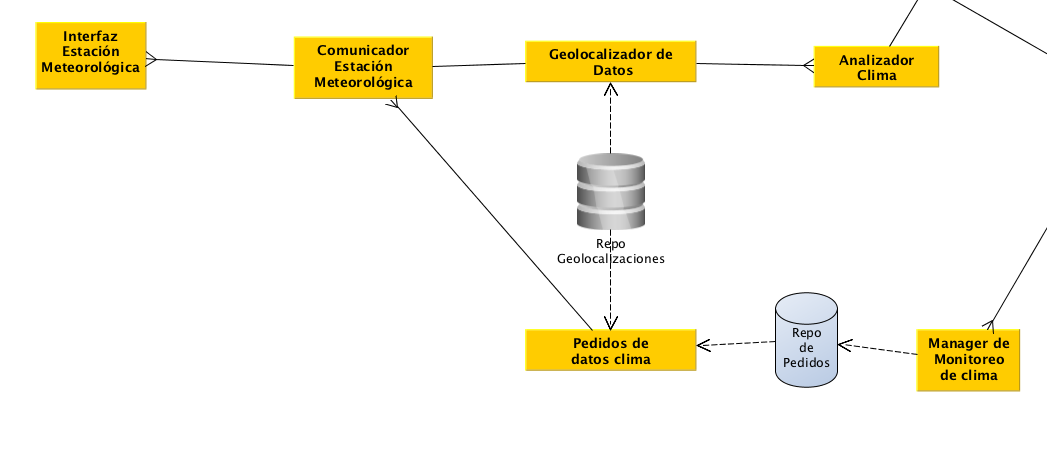
\includegraphics[width=1\textwidth]{./images/arq_clima.png}
  \caption{Arquitectura de comunicación con estaciones meteorológicas y procesamiento de datos}
  \label{fig:clases4}
\end{figure}


\subsection{Comunicación con Interfaz de usuarios}

La interfaz de usuario cuenta con autenticación para asegurar el acceso a la aplicación y un sistema de logging de entradas al sistema para registrar los accesos.

Utilizando la interfaz de usuario, se permite agregar datos sobre las plantaciones de manera manual. También se realiza la configuración de monitoreo de clima y de imágenes (frecuencia, horarios, etc). A su vez, se guarda un log de los cambios en la configuración que se hagan.

El visualizados de datos utiliza la información del repo de datos de plantaciones para mostrar en pantalla el estado actual de las plantaciones.

Por último, el manager de monitoreo de imágenes  y de clima, se encarga de ir agregando los pedidos que deben realizarse para que luego se vayan realizando. Para esto está el repo de pedidos dónde el componente que pide las imágenes se conecta de manera blackboard y luego realiza la solicitud usando el comunicador con los drones.

\begin{figure}[h!]
  \centering
  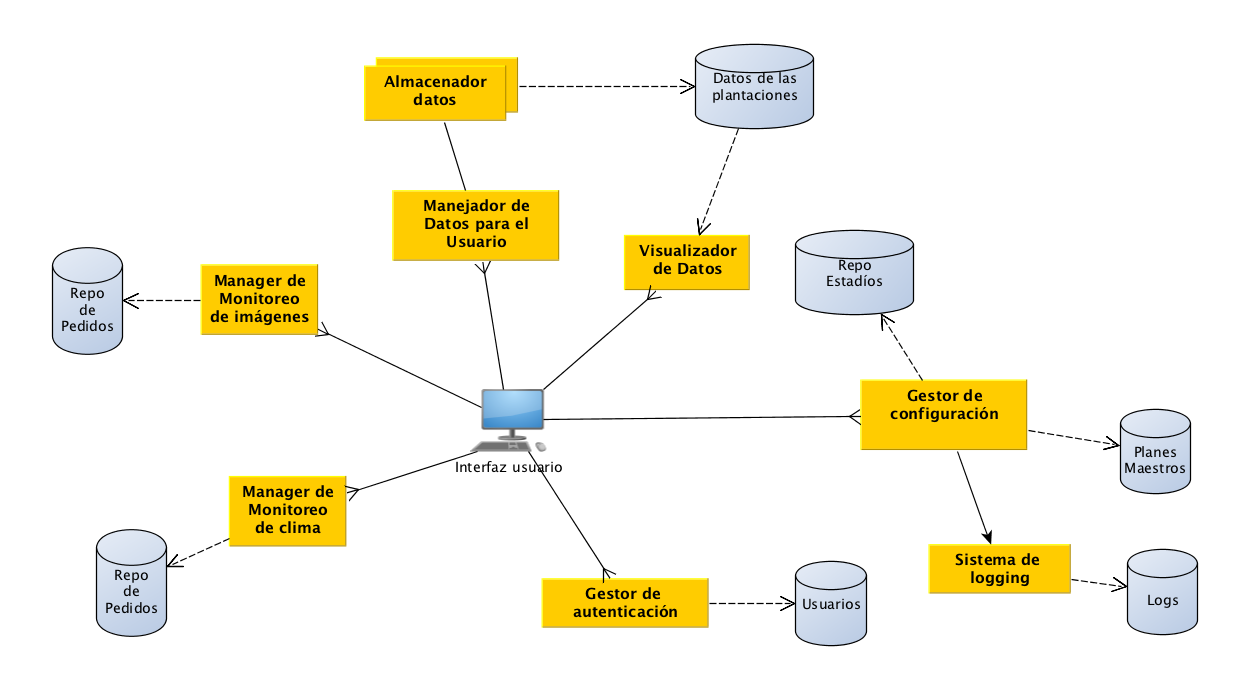
\includegraphics[width=0.8\textwidth]{./images/arq_interfazusuario.png}
  \caption{Arquitectura de comunicación con la interfaz de usuario}
  \label{fig:clases4}
\end{figure}

\subsection{Planificación}

Con la información almacenada en los repositorios, el planificador arma los eventos que deben realizarse para continuar con el plan de trabajo deseado. Luego el manager de actuadores se encarga de enviar el pedido a los distintos actuadores.

Todos los eventos se guardan en un repositorio para permitir la auditabilidad en caso de que sea necesario. 

El controlador de estadiós se encarga de ir cambiando el estado de las plantas en base a los datos que se obtienen y al plan maestro.

\begin{figure}[h!]
  \centering
  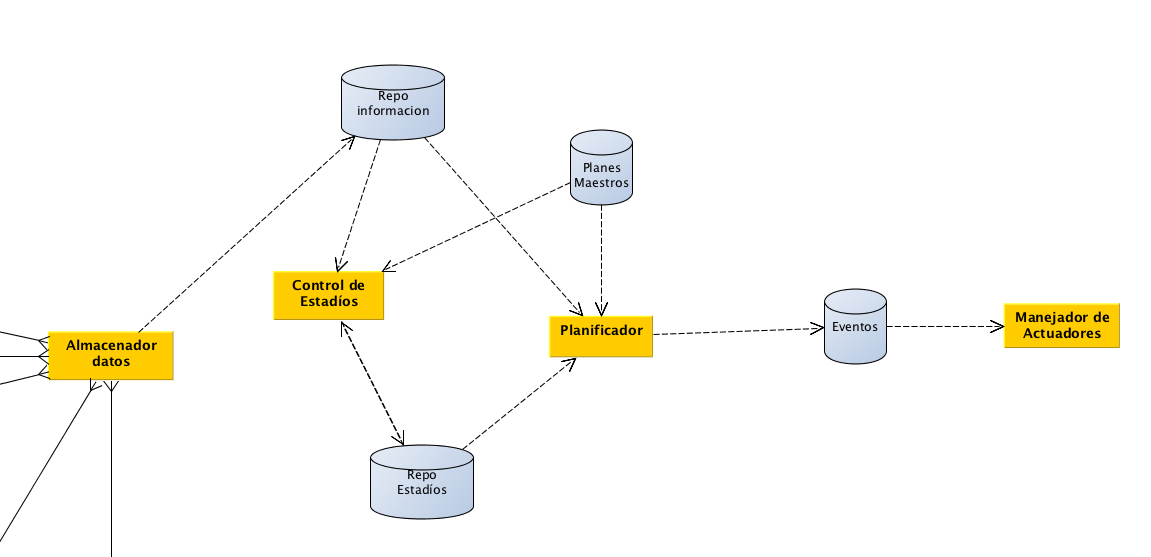
\includegraphics[width=1\textwidth]{./images/arq_plan.png}
  \caption{Arquitectura de planificación de eventos}
  \label{fig:clases4}
\end{figure}

\section{Comparación con el TP1}

De la comparación de las figuras se observa el incremento de complejidad natural al pasar de un entorno controlado y con una sola planta 
a uno con varias plantas distintas, de diferentes tipos y ubicadas en diferentes lugares del país.

En primer lugar observamos que al tener directamente sensores en la tierra no necesitábamos drones para tomar fotos ni componentes para analizar imágenes,
la información sobre el suelo era accesible directamente.

De un modo similar en la comunicación con la interfaz meteorológica evitábamos tener que localizar el lugar de origen de los datos, y nos ahorramos
los componentes específicos para analizar los datos. 

Por otro lado, al haber menor necesidad de guardar información a lo largo del tiempo, hacían falta menos repositorios distribuidos a lo largo de la arquitectura.
El único repositorio de la arquitectura actual que viene de la arquitectura del TP anterior es el de Plan(es) Maestro(s), un concepto que sobrevive todo cambio de
arquitecturas por su importancia en el dominio.
Muchos de los repositorios nuevos que se agregaron tienen que ver con el gran flujo de datos y eventos y la imposibilidad de responder a todos ellos en tiempo real,
algo que en el TP1 no ocurría.

En general vemos que la sucesión de colaboraciones desde la llegada de nueva información hasta el accionar (o no) de los actuadores 
era mucho más simple y corta en el TP1 que en el 2do, presentando componentes con responsabilidades más generales, como los ``Supervisores'' que combina responsabilidades
de que en el TP2 aparecen distribuidas entre la comunicación con los sensores, el analizador de los datos, almacenador, controlador de estadios, planificador, etc.

Sin embargo, si bien las diferencias son variadas y profundas, observamos cierta similitud general entre los diagramas. Algo que podríamos llamar la ``esencia'' de la 
arquitectura permaneció intacto de un TP a otro (aunque casi imposible de visualizar al ojo no entrenado en el dominio del problema). Dicho en términos de la materia,
ambas arquitecturas presentan un estilo similar: existen sensores, el sistema les pide información a esos sensores, la procesa y en función del resultado y de 
lógicas preestablecidas que consulta a partir de repositorios toma decisiones que envía a un conjunto de actuadores que intervienen en el medio de la(s) planta(s).
\section{Conclusiones}
Desde el punto de vista del desarrollo tenemos pocas herramientas para comparar los métodos usados a lo largo de la materia (Scrum y UP),
dado que trabajando con Scrum realizamos una única iteración y trabajando con UP ni siquiera llegamos a desarrollar nada efectivamente.
Además, como cada método lo aplicamos a proyectos de tamaños distintos, la comparación que hagamos estará sesgada por cosas propias de la
complejidad de los problemas que quizás no forman parte de la metodología en sí, entorpeciendo nuestra capacidad de diferenciarlas únicamente
por sus características.

Sin embargo, sí pudimos comparar las etapas iniciales de ambas metodologías, viendo claramente una diferencia entre realizar una planificación
y un diseño antes de comenzar a programar; y empezar a programar sin planificación previa e ir diseñando a medida que se desarrolla. Si bien
en el primer TP consideramos que nuestra aplicación de Scrum era imperfecta pues estábamos acostumbrados a diseñar por adelantado,
en este segundo TP descubrimos que se puede planificar a un nivel más profundo del que conocíamos.

Desde un punto de vista subjetivo, podemos resaltar de UP la priorización de los atributos de calidad como ``drivers'' de las decisiones arquitectónicas,
entendiendo que con Scrum se podrían perder de vista en pos de resolver cuestiones funcionales, y que modificar una aplicación ya construida para que
satisfaga cierto atributo de calidad no contemplado previamente es mucho más costoso que diseñarla teniéndolo en cuenta desde un principio.

Sin embargo, preferimos Scrum a la hora de organizar los tiempos y responsabilidades del proyecto. Como ya dijimos no tuvimos la oportunidad de
experimentarlo nosotros mismos, pero consideramos que, por ejemplo, un error en la estimación de esfuerzo en Scrum tiene consecuencias mínimas
en comparación con las que tendría el mismo error (de estimación de horas/hombre) en UP: en Scrum como mucho una historia quedará afuera de una iteración y
tendrá que ser subdividida más adelante, mientras que en UP puede producir un efecto dominó que afecta todas las iteraciones posteriores
(porque ya se planificaron previamente) y eventualmente postergar todo el proyecto en caso de que la tarea sea crítica.

Entendemos, de todos modos, que combinar las características que destacamos de cada una de las metodologías es no-trivial. Afortunadamente, proponer una metodología
superadora excede el scope de este trabajo práctico.

A la hora de la comparación entre ``programming in the small'' y ``programming in the large'' podemos mencionar la diferencia entre las vistas más usadas: a la hora del 
diseño OO utilizamos tanto diagramas de clases (estático) como de objetos (dinámico) mientras que en la arquitectura se le da más importancia a la vista de
componentes y conectores (dinámica). Creemos que esto tiene que ver con que la arquitectura a gran escala se puede apreciar de manera más simple cuando vemos
cómo estarán los componentes ``en funcionamiento''.

Otra característica distintiva, aunque quizás sea un sesgo de parte de las metodologías usadas, es que la programación a pequeña escala está más orientada
a cumplir con atributos funcionales, mientras en que la programación a gran escala hay que darle mucha más relevancia a cuestiones no funcionales. Esto podría explicarse
si pensamos que en geneneral los productos más grandes son los que tienen más riesgos asociados relacionados con escalabilidad, seguridad, performance, etc.

Desde el punto de vista específico de la realización del trabajo, encontramos dificultades para diferenciar el análisis de riesgos de los atributos de calidad.
En mayor o menor medida, descubrimos que la mayoría de los atributos de calidad tienen algún riesgo relacionado (y viceversa), por lo que por momentos nos 
parecía redundante realizar ambos análisis. Quizás la diferencia se nota mejor en un proyecto real con stakeholders reales en el cual el análisis de riesgos
precede temporalmente a la documentación de atributos de calidad, pero de todos modos encontramos muchos puntos comunes a ambos análisis.


\end{document}
